
\documentclass[12pt]{article}
\usepackage{comment}
\usepackage[utf8]{inputenc}
\usepackage[backend=biber,style=alphabetic,sorting=ynt]{biblatex}
\addbibresource{refs.bib}
\usepackage{xspace}
\usepackage{gastex}
\usepackage{amsmath}
\usepackage{amssymb}
\usepackage{wrapfig}
\usepackage{tikz}
\usepackage{minted}
\usepackage{float}
\usepackage{pgfplots}
\usepackage{booktabs} % For \toprule, \midrule and \bottomrule
\usepackage{pgfplotstable} % Generates table from .csvi
\usepackage{csquotes}
\usepackage{graphicx}
\usepackage{amsmath}
\usepackage{multicol}
\usepackage{tgtermes} % times font
\usepackage[shortlabels]{enumitem}
\usepackage{parskip}

\pagestyle{empty}
\textwidth      165mm
\textheight     252mm
\topmargin      -18mm
\oddsidemargin  -2mm
\evensidemargin -2mm
% \renewcommand{\baselinestretch}{0.96}
\newcommand{\impl}{\mathbin{\Rightarrow}}
\newcommand{\biim}{\mathbin{\Leftrightarrow}}
\newcommand{\id}[1]{\mbox{\textit{#1}}}
\newcommand{\tuple}[1]{\langle #1 \rangle}
\newcommand{\ma}{\mathsf{a}}
\newcommand{\mb}{\mathsf{b}}
\newcommand{\mc}{\mathsf{c}}
\newcommand{\md}{\mathsf{d}}
\newcommand{\nat}{\mathbb{N}}
\newcommand{\intg}{\mathbb{Z}}
\renewcommand*{\bibfont}{\footnotesize}

\newcounter{question}
\newcommand{\question}[1]{
    \stepcounter{question}
    \thequestion. #1 \hfill
}

\newcommand{\revision}[1]{
    \stepcounter{question}
    \thequestion. #1* \hfill
}



\begin{document}
\topskip0pt
\begin{center}
{\sc The University of Melbourne
\\
School of Computing and Information Systems
\\ 
COMP90020 Distributed Algorithms}
\bigskip \\
{\Large\bf Tutorial Week 4: Global States}
\bigskip \\
\end{center}
\section*{Notes}

An event is called \textit{presnapshot} if it occurs at a process before the local snapshot at that process is taken; otherwise it is called \textit{postsnapshot}. A snapshot is consistent if

\begin{itemize}
    \item (1) no postsnapshop event is causally before a presnapshot event
    \item (2) a basic message is included in a channel state if and only if the corresponding send event is presnapshot while the corresponding receive event is postsnapshot.
\end{itemize}



\section*{Exercises}

\setcounter{question}{15}

\question{Consider the following figure:}

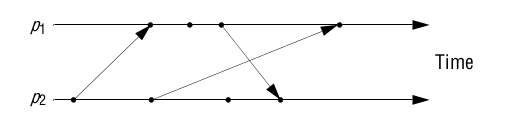
\includegraphics[e]{Tutorial 3/comm.png}

\begin{enumerate}[(a)]
    \item Provide the vector timestamps at each send, receive and concurrent event.
    \item Provide an example of a consistent and inconsistent cut.
\end{enumerate}


\question{Consider the following: Two processes $P$ and $Q$ are connected in a ring using two channels, and they constantly rotate a message $m$. At any one time, there is only one copy of $m$ in the system. Each process’s state consists of the number of times it has received $m$, and $P$ sends $m$ first. At a certain point, $P$ has the message and its state is 102. Immediately after sending $m$, $P$ initiates the snapshot algorithm. Explain the operation of the algorithm in this case, giving the possible global state(s) reported by it.}

\question{Does Chandy-Lamport algorithm work if channels are not FIFO? Provide a counter example or \textbf{show} why it works.}

\question{Argue that a consistent snapshot, meaning one that satisfies properties (1) and (2), rules out orphan messages.}


\end{document}